%遥感专题研究课程论文模板
%带评分选项,可以直接在overleaf上编译,但是需要加入字体
%如果需要添加图片可以自行创一个figures文件夹,小屋内上传不便.
\documentclass[UTF8]{SDAURScourse}
\usetikzlibrary{positioning}
\usetikzlibrary{arrows.meta}
\usetikzlibrary{calc}
\setlength{\absleftindent}{2em} 	%设置摘要缩进
\setlength{\absrightindent}{0pt} 	%设置摘要右边缩进为0
\renewcommand{\abstractname}{} 	%设置摘要名字为空
\graphicspath{{figures/}}

\Chtitle{机器学习在遥感中的应用}			%中文题目
\Entitle{机器学习在地球科学中的应用}		%翻译题目	
\fdate{2019-2020-2}										%第一行
\name{种田人}											%姓名
\studentnumber{20177740}					%学号
\session{2017}										%届数
\major{遥感科学与技术}						%专业
\class{2}												%班级
\ldate{二 0 二 0 年 \ 7月  \  13 日}		%学院下面的日期

%分数老师填写
\scorea{90}
\scoreb{90} 
\scorec{90}
\scored{90}

\begin{document}

%生成封面页
\makecover		

%摘要页
% !TEX encoding = UTF-8
%自行在相应位置填上内容

%第一页开始
\title{\songti \bfseries \zihao{2} 机器学习在遥感中的应用}
\author{\fangsong \zihao{-3} 种田人 \\ { \zihao{5}17级遥感科学与技术 2班}}
\date{}

%生成标题
\maketitle

%题目	
\begin{center}
	\zihao{-3} {\bfseries machine learning in remote sensing}  \\[0.2pt]
	{\zihao{-4} ZhongTian er}
\end{center}

%中文摘要     
\begin{onecolabstract}
	\vspace{-3em}
	\noindent{}{\bfseries \zihao{-5}摘要:}  这里是中文摘要,这里是中文摘要,这里是中文摘要,这
	里是中文摘要,这里是中文摘要。  \\
	\noindent{}{{{\bfseries \zihao{-5} 关键词:}}机器学习;遥感;算法;应用}   
\end{onecolabstract}
%英文摘要
\begin{onecolabstract}
	\vspace{-2.8em}
	\noindent{}{\bfseries \zihao{-5} Abstract:} This is an abstract, This is an abstract,This is an 
	abstract,This is an abstract.\\
	\noindent{}{{\bfseries \zihao{-5} Keywords:} Machine learning; Remote sensing; Alogrithm;Applications}
\end{onecolabstract}

%第一节
% !TEX encoding = UTF-8
\section{导言}
这里是导言,这里是导言,这里是导言。这里是导言,这里是导言,这里是导言。这里是导
言,这里是导言,这里是导言。这里是导言,这里是导言,这里是导言。这里是导言,这里
是导言,这里是导言。这里是导言,这里是导言,这里是导言。这里是导言,这里是导言,
这里是导言。这里是导言,这里是导言,这里是导言。这里是导言,这里是导言,这里是导
言。这里是导言,这里是导言,这里是导言。这里是导言,这里是导言,这里是导言。
%第一章
\section{机器学习}
\subsection{什么是机器学习}
%什么是机器学习
\par 
什么是机器学习,什么是机器学习,什么是机器学习,什么是机器学习什么是机器学习,什
么是机器学习什么是机器学习,什么是机器学习什么是机器学习,什么是机器学习什么是机
器学习,什么是机器学习什么是机器学习,什么是机器学习什么是机器学习,什么是机器学
习\cite{机器学习技术的应用经验及建议探讨}。

%机器学习算法
\subsection{常见的机器学习方法}
%K-means算法
\subsubsection{K-means算法}
\par 
K-means,K-means,K-means,K-means,K-means,K-means,K-means,K-means,K-means,K-means,K-me
ans,K-means,K-means,K-means,K-means,K-means,
%聚类是非监督学习的一种形式,它将一个观测集(即数据点)划分到孜然组合或者模式划分到
自然组或者模式聚类,聚类的途径是测量分配给每个聚类的观测对之间的相似性以最小一个指
定的代价函数\cite{Simon2011神经网络与机器学习}。

\begin{equation}
	C\left(i\right) = arg \min_{i \le j \le K}    \Vert \mathbf{x_i}  - \hat{\mathbf{\mu_j}} \Vert^{2}  
\end{equation}
	
%%tikz绘图
\begin{figure}[h]
	\centering
	\begin{tikzpicture}
		\node (ciji)  [] at (-0.5,0) {刺激};
		\node (ganshouqi)[draw,minimum height = 0.8cm,thick] at (1.5,0)  {感受器};
		\node (shenjing)    [draw,minimum height = 0.8cm,thick]  at (4,0) {神经网络};
		\node (xiaoying)   [draw,minimum height = 0.8cm,thick] at (6.5,0) {效应器};
		\node (xiangying) [minimum height = 0.8cm,thick] at (8.5,0) {响应};
		\draw [-Stealth]  (ciji.east) -- (ganshouqi.west);
		\draw [-Stealth] (2.172,0.2) -- (3.146,0.2);
		\draw [-Stealth] (3.146,-0.2) -- (2.172,-0.2);
		\draw [-Stealth] (4.87,0.2) -- (5.83,0.2);
		\draw [-Stealth] (5.83,-0.2) -- (4.87,-0.2);
		\draw [-Stealth] (xiaoying.east) -- (xiangying.west); 
	\end{tikzpicture}
	\caption{神经系统}
	\label{neutural network}
\end{figure}

\begin{figure}[htbp]
	\centering
	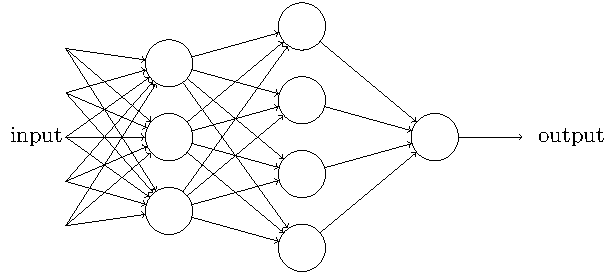
\includegraphics{Neural Networks-pic1.pdf}
	\caption{神经网络}
	\label{Neural Networks}
\end{figure}



%第二节
% !TEX encoding = UTF-8

	%遥感部分
		\section{遥感}	
		\subsection{什么是遥感}
		\par 
		遥感是指在不直接接触的情况下,在地面,高空和外层空间的各种平台上,运用各种传感器
		获取各种数据,通过传输,变换和处理,提取有用的信息,实现研究地物空间形态、位置、性
		质、变化及其与环境的关系的一门现代应用技术学科\cite{孙家柄2009遥感原理与应用}
		。
		遥感具有探测范围广、光谱探测范围大、快速周期成像、经济效益高等特点。使得它在
		军事、农业、城市规划、灾害检测、资源探查领域有广泛的应用。


%第三节
\include{ection4}

%参考文献bib
\bibliography{reference}


\end{document}